\documentclass{beamer}
\usepackage[utf8]{inputenc}
\usepackage{amsmath}
\usepackage{graphicx}
\usepackage{xcolor}
\usepackage{tikz}

\usetheme{Madrid}
\usecolortheme{default}

% Define custom colors inspired by Star Trek DS9
\definecolor{ds9blue}{RGB}{25,25,112} % Midnight Blue
\definecolor{ds9gold}{RGB}{218,165,32} % Goldenrod
\definecolor{ds9grey}{RGB}{105,105,105} % Dim Gray
\definecolor{ds9red}{RGB}{178,34,34} % Firebrick

% Customize the colors
\setbeamercolor{title}{fg=ds9gold}
\setbeamercolor{frametitle}{bg=ds9blue, fg=white}
\setbeamercolor{block title}{bg=ds9gold, fg=black}
\setbeamercolor{block body}{bg=ds9grey!20, fg=black}
\setbeamercolor{section in toc}{fg=ds9gold}
\setbeamercolor{subsection in toc}{fg=ds9gold!70}
\setbeamercolor{footline}{bg=ds9blue, fg=white}
\setbeamercolor{author in head/foot}{fg=white}
\setbeamercolor{date in head/foot}{fg=white}
\setbeamercolor{title in head/foot}{fg=white}

% Title page configuration
\title[Unit 2 Review]{PHYS12 CH459:}
\subtitle{Test Prep}
\author[Mr. Gullo]{Mr. Gullo}
\date[Nov 2024]{November 2024}

% Add logo
\logo{
\includegraphics[width=0.1\linewidth]{phys12-shared-cinec-logo.png}}

% Table of contents at the beginning of each section
\AtBeginSection[]
{
  \begin{frame}
    \frametitle{Table of Contents}
    \tableofcontents[currentsection]
  \end{frame}
}


\begin{document}

\frame{\titlepage}


\section{Circus Performer Problem}

\begin{frame}
\frametitle{Problem 1: Circus Performance}
\begin{block}{Problem Statement}
During a circus act:
\begin{itemize}
    \item One performer hangs upside down from trapeze
    \item Holds another performer by the legs
    \item Upward force is three times the lower performer's weight
    \item Calculate the stretch in the upper legs (femurs)
\end{itemize}
\end{block}
\begin{figure}
    \centering
    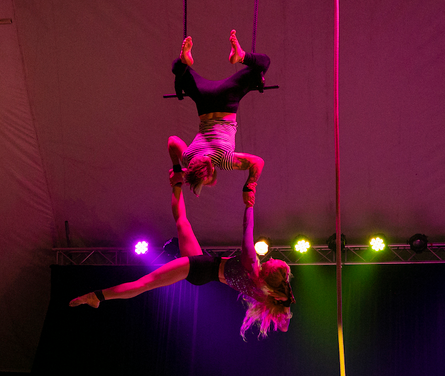
\includegraphics[width=0.5\linewidth]{CH9.5 4,5,9 Review/Screenshot 2024-11-12 100229.png}
\end{figure}

\end{frame}

\begin{frame}
\frametitle{Problem 1: Given Information}
\begin{itemize}
    \item Mass of performer = 60.0 kg
    \item Each femur:
    \begin{itemize}
        \item Length ($L_0$) = 35.0 cm = 0.350 m
        \item Radius = 1.80 cm = 0.0180 m
    \end{itemize}
    \item Young's modulus ($Y$) = $1.6 \times 10^{10}$ N/m²
    \item Force = 3 times weight
\end{itemize}
\end{frame}

\begin{frame}
\frametitle{Problem 1: Solution Approach}
Key equation for elastic deformation:
$$\Delta L = \frac{1}{Y} \frac{F}{A} L_0$$
where:
\begin{itemize}
    \item $\Delta L$ = change in length
    \item $Y$ = Young's modulus
    \item $F$ = applied force
    \item $A$ = cross-sectional area
    \item $L_0$ = original length
\end{itemize}
\end{frame}

\begin{frame}
\frametitle{Problem 1: Calculations}
\begin{enumerate}
    \item Calculate total force:
    $$F_{\text{tot}} = 3mg = 3(60.0\text{ kg})(9.80\text{ m/s}^2) = 1764\text{ N}$$
    \item Force per leg:
    $$F_{\text{leg}} = F_{\text{tot}}/2 = 882\text{ N}$$
    \item Cross-sectional area:
    $$A = \pi r^2 = \pi(0.0180\text{ m})^2 = 1.018 \times 10^{-3}\text{ m}^2$$
\end{enumerate}
\end{frame}

\begin{frame}
\frametitle{Problem 1: Final Result}
Substituting into the equation:
$$\Delta L = \frac{1}{1.6 \times 10^{10}\text{ N/m}^2} \frac{882\text{ N}}{1.018 \times 10^{-3}\text{ m}^2}(0.350\text{ m})$$
$$\Delta L = 1.90 \times 10^{-5}\text{ m}$$
Or in centimeters:
$$\Delta L = 1.90 \times 10^{-3}\text{ cm}$$
\end{frame}

\section{Aircraft Towing Problem}

\begin{frame}
\frametitle{Problem 2: Aircraft Towing}
\begin{block}{Problem Statement}
A tractor pushes an airplane:
\begin{itemize}
    \item Tractor mass = 1800 kg
    \item Force on pavement = $1.75 \times 10^4$ N backward
    \item Total resistance = 2400 N
    \item Acceleration = 0.150 m/s²
\end{itemize}
Find: (a) airplane mass, (b) force on airplane
\end{block}
\end{frame}
\begin{frame}
\begin{figure}
    \centering
    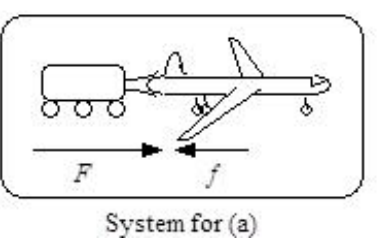
\includegraphics[width=0.5\linewidth]{CH9.5 4,5,9 Review/Screenshot 2024-11-12 092937.png}
\end{figure}
\begin{figure}
    \centering
    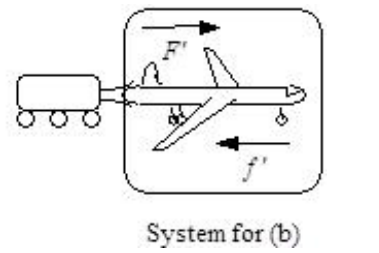
\includegraphics[width=0.5\linewidth]{CH9.5 4,5,9 Review/Screenshot 2024-11-12 092940.png}
    
\end{figure}
\end{frame}

\begin{frame}
\frametitle{Problem 2: Solution Part (a)}
Using Newton's Second Law:
\begin{align*}
\text{net }F &= Ma = (m_a + m_t)a = F - f\\
m_a &= \frac{F-f}{a} - m_t\\
m_a &= \frac{1.75 \times 10^4\text{ N} - 2400\text{ N}}{0.150\text{ m/s}^2} - 1800\text{ kg}\\
m_a &= 9.89 \times 10^4\text{ kg}
\end{align*}
\end{frame}

\begin{frame}
\frametitle{Problem 2: Solution Part (b)}
Force on airplane:
\begin{align*}
\text{net }F &= F' - f' = m_aa\\
F' &= m_aa + f'\\
F' &= (9.89 \times 10^4\text{ kg})(0.150\text{ m/s}^2) + 2200\text{ N}\\
F' &= 1.70 \times 10^4\text{ N}
\end{align*}\end{frame}



\section{Car Acceleration Problem}

\begin{frame}
\frametitle{Problem 3: Car Acceleration}
\begin{block}{Problem Statement}
A car accelerates forward:
\begin{itemize}
    \item Wheels exert 2100 N backward on road
    \item Friction force = 250 N
    \item Acceleration = 1.80 m/s²
\end{itemize}
Find the mass of car plus occupants
\end{block}
\end{frame}

\begin{frame}
\frametitle{Problem 3: Solution}
Using Newton's Second Law:
\begin{align*}
\text{net }F &= F - f = ma\\
m &= \frac{F-f}{a}\\
m &= \frac{2100\text{ N} - 250\text{ N}}{1.80\text{ m/s}^2}\\
m &= 1.03 \times 10^3\text{ kg}
\end{align*}
\begin{figure}[H]
    \centering
    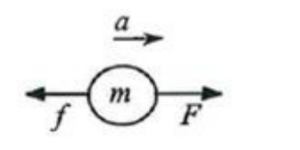
\includegraphics[width=0.5\linewidth]{CH9.5 4,5,9 Review/Screenshot 2024-11-12 092952.png}
\end{figure}

\end{frame}

\begin{frame}
\frametitle{Key Takeaways}
\begin{itemize}
    \item Elastic deformation depends on material properties and geometry
    \item Newton's laws apply to complex systems like aircraft-tractor combinations
    \item Free-body diagrams help organize force analysis
    \item Always check units and magnitudes for reasonable results
\end{itemize}
\end{frame}

\begin{frame}
\frametitle{Problem: Forces on Head at Drafting Board}
\begin{block}{Problem Statement}
A person working at a drafting board holds her head at an angle:
\begin{itemize}
    \item Three major forces act on the head:
    \begin{itemize}
        \item Weight ($w$) = 50.0 N
        \item Muscle force ($F_M$) = 60.0 N at 33°
        \item Vertebrae force ($F_V$) at unknown angle $\theta$
    \end{itemize}
    \item All forces act through center of mass
    \item Head is stationary (in equilibrium)
\end{itemize}
Find direction ($\theta$) and magnitude of vertebrae force ($F_V$).
\end{block}
\begin{figure}
    \centering
    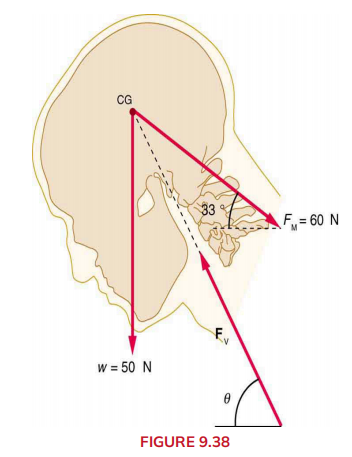
\includegraphics[width=0.2\linewidth]{CH9.5 4,5,9 Review/Screenshot 2024-11-11 143247.png}
\end{figure}

\end{frame}

\begin{frame}
\frametitle{Solution Approach}
\begin{itemize}
    \item Since head is stationary, sum of forces = 0
    \item Break forces into x and y components:
    \begin{align*}
    \hat{x}&: F_M \cos 33° = F_V \cos \theta\\
    \hat{y}&: w + F_M \sin 33° = F_V \sin \theta
    \end{align*}
    \item Use these equations to find $\theta$ and $F_V$
\end{itemize}
\begin{figure}
    \centering
    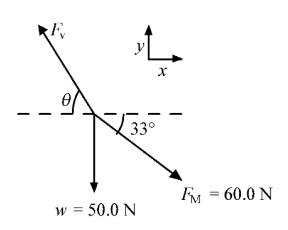
\includegraphics[width=0.5\linewidth]{CH9.5 4,5,9 Review/Screenshot 2024-11-12 103435.png}
\end{figure}

\end{frame}

\begin{frame}
\frametitle{Solution: Finding the Angle}
\begin{itemize}
    \item Divide y-equation by x-equation to find $\theta$:
    \[\tan \theta = \frac{w + F_M \sin 33°}{F_M \cos 33°}\]
    \item Substitute known values:
    \[\tan \theta = \frac{50.0\text{ N} + (60.0\text{ N})\sin 33°}{(60.0\text{ N})\cos 33°} = 1.643\]
    \item Solve for $\theta$:
    \[\theta = \tan^{-1}(1.643) = 58.7° \approx 59°\]
\end{itemize}
\end{frame}

\begin{frame}
\frametitle{Solution: Finding the Force Magnitude}
\begin{itemize}
    \item Use x-component equation:
    \[F_V = \frac{F_M \cos 33°}{\cos 58.7°}\]
    \item Substitute values:
    \[F_V = \frac{(60.0\text{ N})\cos 33°}{\cos 58.7°} = 97\text{ N}\]
    \item Therefore:
    \begin{itemize}
        \item Direction: $\theta = 59°$ from horizontal
        \item Magnitude: $F_V = 97$ N
    \end{itemize}
\end{itemize}
\end{frame}

\begin{frame}
\frametitle{Physical Interpretation}
\begin{itemize}
    \item The vertebrae must supply a significant force (97 N) to maintain head position
    \item Force is nearly 2 times the weight of the head
    \item Angle is determined by:
    \begin{itemize}
        \item Head position (33° muscle angle)
        \item Need to balance both vertical and horizontal components
        \item Requirement that force passes through center of mass
    \end{itemize}
    \item Demonstrates why poor posture can lead to muscle strain
\end{itemize}
\end{frame}




\begin{frame}
\frametitle{Problem: Leg Exercise Device}
\begin{block}{Problem Statement}
An exercise device for the upper leg muscle:
\begin{itemize}
    \item Mass of 10.0 kg attached via pulleys
    \item System maintained at constant speed
    \item Lever arm distances:
    \begin{itemize}
        \item $r_\perp = 35.0$ cm (perpendicular distance to tension force)
        \item $r'_\perp = 2.00$ cm (perpendicular distance to muscle force)
    \end{itemize}
\end{itemize}
Calculate the force exerted by the upper leg muscle.
\end{block}
\begin{figure}
    \centering
    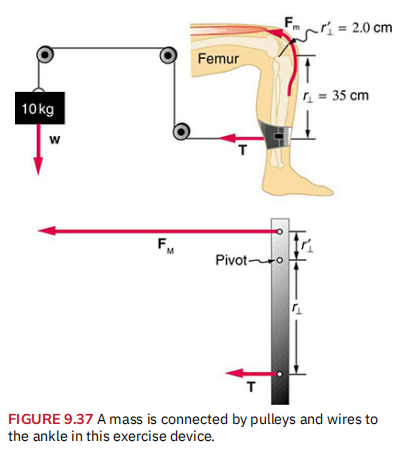
\includegraphics[width=0.5\linewidth]{CH9.5 4,5,9 Review/Screenshot 2024-11-12 134327.png}
\end{figure}
\end{frame}

\begin{frame}
\frametitle{Analysis Strategy}
Key physics concepts:
\begin{itemize}
    \item Constant speed implies:
    \begin{itemize}
        \item Acceleration $a = 0$
        \item Net force = 0
        \item Net torque $\tau = 0$
    \end{itemize}
    \item Torque relationship:
    \begin{itemize}
        \item $\tau = F r_\perp$ (force × perpendicular distance)
        \item Sum of torques = 0 for equilibrium
    \end{itemize}
\end{itemize}
\end{frame}

\begin{frame}
\frametitle{Solution Steps}
\begin{enumerate}
    \item Calculate tension force from weight:
    \[T = w = (10.0\text{ kg})(9.80\text{ m/s}^2) = 98.0\text{ N}\]
    \item Use torque equilibrium about pivot:
    \[F_m r'_\perp - T r_\perp = 0\]
    \item Solve for muscle force:
    \[F_m = T\frac{r_\perp}{r'_\perp}\]
\end{enumerate}
\end{frame}

\begin{frame}
\frametitle{Final Calculation}
Substituting values:
\begin{align*}
F_m &= 98.0\text{ N} \times \frac{35.0\text{ cm}}{2.00\text{ cm}}\\
&= 98.0\text{ N} \times 17.5\\
&= 1715\text{ N}\\
&= 1.72 \times 10^3\text{ N}
\end{align*}
\end{frame}

\begin{frame}
\frametitle{Physical Interpretation}
\begin{itemize}
    \item The muscle must exert a force of 1715 N 
    \item This large force results from mechanical disadvantage:
    \begin{itemize}
        \item Muscle attachment point (2.00 cm) much closer to pivot
        \item Than weight attachment point (35.0 cm)
        \item Creates a force multiplier of 17.5
    \end{itemize}
    \item Demonstrates why leg muscles need to be very strong
    \item Shows importance of lever arms in biomechanics
\end{itemize}
\end{frame}


\end{document}